\documentclass{article}

% Page margins
\usepackage[top=1in, bottom=1in, left=1in, right=1in]{geometry}

% Required for biblatex
\usepackage{csquotes}  

% Math & formatting
\usepackage{amsmath}
\usepackage{appendix}
\usepackage{microtype}
\usepackage{graphicx}
\usepackage{placeins}
\usepackage{subcaption}
\usepackage{indentfirst}
\usepackage{longtable}
\usepackage{tikz}
\usetikzlibrary{shapes, arrows.meta, positioning, calc}
\usepackage{float}
\usepackage{booktabs}
\usepackage{adjustbox}
\usepackage{newunicodechar}
\newunicodechar{≥}{\geq}

% Correct biblatex loading (DO NOT load inputenc if XeLaTeX)
\usepackage[style=authoryear, backend=biber, sorting=nyt]{biblatex}
\addbibresource{references.bib}

\title{Encoding Emotion in Music via Acoustic Features:\\
A Weakly Supervised Machine Learning Study}
\author{Jiaming Mao \\ University of Chicago \\ 
\texttt{jmao0220@uchicago.edu}}
\date{May 2025}

\setlength{\parskip}{0.8em}
\setlength{\parindent}{0pt}

\begin{document}

\maketitle

\begin{abstract}
This study investigates how accurately and interpretably machine learning models can classify emotional content in music using only Spotify-derived acoustic features. Over 80,000 tracks were weakly labeled with six basic emotions—\textit{joy}, \textit{sadness}, \textit{anger}, \textit{disgust}, \textit{fear}, and \textit{surprise}—by applying a transformer-based classifier (DistilRoBERTa) to Last.fm user-generated tags. A top-$k$ multilabel evaluation strategy was used to reflect the non-exclusive nature of musical emotion.

Three models—Random Forest, K-Nearest Neighbors, and Multi-Layer Perceptron—were trained and compared. Random Forest achieved the highest micro-average F1 score (0.690) and exact match accuracy (38.77\%), outperforming others particularly in precision on low-frequency classes like \textit{fear} and \textit{disgust}. However, some emotion categories remained difficult to separate due to co-occurrence and semantic ambiguity.

Feature importance comparisons revealed that \texttt{acousticness}, \texttt{energy}, \texttt{valence}, and \texttt{loudness} contributed most to emotional inference, while features like \texttt{mode} and \texttt{key} had limited value. SHAP-based interpretation showed that errors often stemmed from low signal strength or conflicting feature cues rather than random noise. Ablation studies confirmed that emotional prediction is driven by a compact yet expressive acoustic subspace.

Limitations include reliance on transformer-generated labels, absence of lyrical features, and potential genre-specific biases. Still, the findings demonstrate the feasibility of weakly supervised, audio-based multilabel emotion recognition and provide interpretable insight into how models learn affect from music.
\end{abstract}


\section{Introduction}
    
Music has long been recognized as a powerful conduit for emotional expression, and its ability to evoke affective responses is deeply embedded in both biological and cultural dimensions \parencite{Huron2015, Perlovsky2010}. Computational models have increasingly attempted to classify emotional responses to music by analyzing audio features such as tempo, timbre, energy, and spectral properties. Although model performance (e.g. accuracy, F1 score) remains a common evaluation focus \parencite{Yang2024, Yoo2024}, the recent literature suggests a more nuanced perspective: different machine learning models vary not only in prediction performance but also in their sensitivity to different musical features \parencite{Xia2022, Xu2011}.

This paper investigates the question: \textit{How accurately can supervised machine learning models predict user-assigned emotional categories of songs using only audio features, and which audio features contribute most to these predictions?} Rather than simply comparing which model performs best, the objective is to examine how models such as Random Forest, MLP, and KNN use characteristics differently to make predictions. This approach is motivated by recent findings that indicate that the effectiveness of features such as MFCCs, energy, roll-off, and pitch can vary substantially between models \parencite{Juthi2020, Rosner2018, Garg2022}. Some models may rely more on spectral sharpness or rhythm, while others may favor dynamic or harmonic information. Understanding these patterns helps clarify both the behavior of models and the nature of musical emotion itself.

The theoretical foundation for this investigation comes from emotion models such as Russell's circumplex model and Thayer's valence arousal plane \parencite{Helmholz2019}, as well as psychological studies on how acoustic features induce affect \parencite{McCraty1998, Leubner2017}. Furthermore, my study builds on the literature on domain-specific emotion recognition, particularly research integrating lyrics or domain-tuned lexicons \parencite{Bandhakavi2017, Xu2011}. These works suggest that interpretability and modality-specific contributions are essential for building robust, generalizable emotional classifiers.

By analyzing feature importance rankings across classifiers and exploring areas of agreement and divergence, this paper offers a new perspective on model interpretability in music emotion recognition. The goal is not only to identify which features predict emotion best, but to ask \textit{why certain features matter more to some models than others}, and what this implies for both machine learning research and affective music theory.

Specifically, this study makes the following contributions:

\begin{itemize}
    \item It constructs a weakly labeled dataset of over 80,000 songs by mapping Last.fm tags to emotion categories using a transformer-based semantic model (DistilRoBERTa), enabling large-scale training without manual annotation.
    \item It systematically compares how three classifiers—Random Forest, K-Nearest Neighbors, and MLP—use acoustic features to predict emotional categories, highlighting both performance trade-offs and distinct model-specific feature importances.
    \item It introduces a multi-perspective interpretability framework including permutation-based feature attribution, SHAP analysis, and error-driven model interpretation, offering practical insights into classifier behavior and emotion-specific confusion.
\end{itemize}


\section{Literature Review}

This study builds on multiple strands of prior research, drawing on theories of emotional structure, semantic projection from social tagging systems, machine learning models for text-based emotion detection, acoustic feature analysis in music information retrieval (MIR), and model interpretability techniques. Together, these literatures inform the construction of our labeling pipeline, the design of our audio-based classifiers, and our strategy for interpreting feature contributions.

\subsection{Theoretical Models of Emotion Representation}

Understanding emotion begins with selecting a representational framework that captures the complexity of affective states. Russell's Circumplex Model \parencite{Russell1982}, which characterizes emotion in a two-dimensional valence-arousal space, remains foundational in both psychological and MIR research. Its strength lies in expressing subtle gradients between emotions rather than reducing them to discrete categories. Recent studies, such as Longo et al. (2024), reaffirm the model’s generalizability across multimodal contexts, demonstrating that textual, auditory, and visual expressions of emotion continue to cluster meaningfully within the valence-arousal plane \parencite{Longo2024}. These findings support the choice of emotion-related features like energy and danceability in this project, which serve as valence-arousal proxies for downstream prediction.

\subsection{Challenges in Music Emotion Annotation}

Accurate labeling of music emotion data remains a central challenge in MIR. Manual annotation is prohibitively expensive and often inconsistent, as emphasized by Cano and Schuller (2017), who note that high-quality labeled datasets are rare \parencite{Cano2017}. To address this, researchers increasingly turn to user-generated metadata such as Last.fm tags, which offer a noisy but scalable alternative. The challenge, however, is to translate these free-text tags into reliable emotion labels. While previous studies such as Olha et al. (2023) have proposed using word embeddings like Word2Vec for semantic clustering of tags \parencite{Olha2023}, this study adopts a more context-aware approach by applying a transformer-based zero-shot classifier (DistilRoBERTa) to map tags directly to emotion categories. This strategy better handles polysemous or stylistically nuanced tags and enables large-scale emotion labeling without relying on rigid keyword lists.


\subsection{Music Information Retrieval and Acoustic Feature Relevance}

Content-based MIR provides the foundation for choosing acoustic features that relate to emotional perception. Casey et al. (2008) identify a wide range of relevant features—from timbral texture to rhythm and pitch—that help structure automated MIR systems \parencite{Casey2008}. Building on this, Kamenetsky et al. (1997) conducted psychological experiments revealing that musical parameters such as tempo and intensity reliably shift emotional perception \parencite{Kamenetsky1997}. These findings support the idea that low-level audio features can encode high-level affective meaning, making them well-suited for use as inputs in emotion-predictive models.

\subsection{Semantic Labeling Using Transformer-Based Language Models}

To improve the semantic labeling of noisy, user-generated text inputs, transformer-based models such as BERT, RoBERTa, and their distilled variants provide significant advantages. Unlike static embedding models, transformers can capture contextual nuance in short and ambiguous tags through self-attention mechanisms. Acheampong et al. (2021) synthesize findings across domains and show that transformer models outperform traditional approaches on short-text classification tasks, a common characteristic of Last.fm tags \parencite{Acheampong2021}. In the specific context of music tagging, \textcite{Olha2023} demonstrate that RoBERTa maintains high classification accuracy even when applied to semantically fuzzy or stylistically diverse user labels. Building on this evidence, this study implemented DistilRoBERTa as the core tagging model, allowing for fine-grained emotion classification while retaining scalability. This approach enables the system to assign emotional categories such as \textit{fear} or \textit{surprise} to compound or metaphorical tags like \texttt{trippy jazz} or \texttt{dark nostalgia}—cases where static models often fail. Recent work by \textcite{Artemova2025} further validates the use of transformer-generated labels, showing that minimal human review of LLM outputs can rival or exceed traditional crowd-annotation, especially in subjective domains like emotion recognition. Similarly, \textcite{Kim2024} show that prompt-engineered transformers can successfully classify real-world, weakly structured inputs, such as open-ended student responses in educational settings. These developments collectively justify the use of transformer-based pipelines as robust tools for weak supervision in emotion classification tasks.


\subsection{Weak Supervision and Label Quality Considerations}

Weak supervision techniques are essential in large-scale emotion classification tasks where human-annotated ground truth is impractical to obtain. In affective computing and educational research, label proxies—such as semantic projections or model-generated tags—are increasingly accepted, provided they are transparently validated. Kim et al. (2024) present a powerful example of this approach through a human-centered LLM-integrated dashboard for writing education, where ChatGPT-based feedback and behavior logs are automatically analyzed using fine-tuned models \parencite{Kim2024}. Their system detects misuse patterns, aligns student inputs with curricular learning objectives, and enables teachers to provide adaptive feedback based on weakly supervised signals derived from chat data and model predictions. This reinforces the feasibility of using LLM-generated labels, especially when paired with targeted human oversight. Inspired by their methodology, this study treats Last.fm tag-derived emotion labels as a form of distant supervision, acknowledging their noise but leveraging semantic embeddings to minimize inconsistency. Kim et al.’s design also underscores the importance of involving end users (in their case, teachers) in refining model interpretations—paralleling our inclusion of interpretable model diagnostics to mitigate label-induced bias. Their iterative process, combining NLP expertise with qualitative insights, sets a methodological precedent for managing noisy data pipelines in emotion-related applications. While risks such as semantic drift and confirmation bias remain, their work provides a practical blueprint for transparent and human-aligned weak supervision systems, validating the broader use of model-based labeling in complex, subjective domains like musical emotion classification. Importantly, \textcite{Tuba2025} demonstrate that even in the absence of gold-standard annotations, weakly supervised pipelines using rule-based emotion taggers and acoustic feature heuristics can achieve strong multi-label classification results. Their hybrid model, evaluated on genre-diverse music corpora, supports the viability of scalable labeling strategies when human annotation is infeasible. These findings align with the approach taken in this study: leveraging transformer-based emotion projections on Last.fm tags as a proxy for listener affect across a broad corpus of songs.


\subsection{Multi-Label Emotion Classification in Music}

Affective responses to music are inherently multidimensional: a single track may evoke joy and nostalgia simultaneously, or anger interlaced with excitement. Capturing this complexity requires moving beyond traditional single-label classification. Multi-label frameworks allow each musical input to be associated with a set of emotional categories, better reflecting real-world listening experiences. Ahsan, Kumar, and Jawahar (2015) frame music annotation as a multi-label classification task and compare algorithms such as binary relevance, classifier chains, and ensemble methods, finding that multi-label models outperform one-hot emotion classifiers in expressive range and precision. More recently, Uplabdhee et al. (2025) provide a comprehensive evaluation of multi-label music emotion recognition using deep neural networks and rule-based heuristics, emphasizing that multi-label output not only improves classification metrics but also aligns more closely with psychological models of emotion. Their study reveals that incorporating co-occurrence information and feature-level fusion enhances both recall and emotional plausibility. This study adopts the same perspective, implementing a top-$k$ dynamic matching strategy to allow each track to receive multiple emotional predictions. This design choice reflects both empirical success in recent literature and theoretical alignment with the non-exclusive nature of emotional expression in music.



\subsection{Interpretability of Machine Learning Models in Emotion Prediction}

Interpretability methods are essential for understanding the behavior of black-box models in emotion classification. As Parthasarathy et al. (2017) argue, accurate predictions alone are insufficient without insight into which features drive these predictions \parencite{Parthasarathy2017}. Tools like SHAP values and permutation importance help quantify individual feature contributions, improving transparency. Though initially developed in contexts like fraud detection, these methods translate effectively to MIR applications. This study applys permutation feature importance to assess which acoustic features most strongly influence model outputs, ensuring that emotion predictions remain interpretable and aligned with psychological theories of affect. Kim et al. (2024) similarly advocate for interpretability in educational AI tools, showing that teachers rely on NLP-enhanced dashboards to gain contextual and semantic insights into student behavior, rather than relying on statistical summaries alone \parencite{Kim2024}. Their approach strengthens the case for embedding interpretability at every level of the modeling pipeline in subjective domains like emotion.

Together, these strands of literature provide both the conceptual and methodological foundations for the current study. The following section describes how these theories were operationalized into a data labeling pipeline and feature-driven classification framework.

\section{Data and Methods}

\subsection{Dataset Construction and Emotion Labeling}

This study investigates how machine learning models classify songs into emotional categories based on audio features extracted from Spotify. The emotion labeling pipeline begins with user-generated tags from the Last.fm subset of the Million Song Dataset \parencite{MillionSongDataset}, which includes two primary SQLite files: \texttt{tags.db}, containing user-assigned tags for tracks and their IDs, and \texttt{track\_metadata.db}, containing track metadata including track ID, name, and artist. The final dataset includes over 80,000 songs labeled with one or more of six emotions and enriched with Spotify-derived audio features. The pipeline proceeds as follows:

\paragraph{Tag-to-Emotion Mapping.}

To generate emotion labels from Last.fm’s user-generated tags, this study adopted a transformer-based model: DistilRoBERTa fine-tuned for multi-class emotion classification \parencite{Hartman2022}. Compared to static embeddings, DistilRoBERTa captures contextual meaning by leveraging attention-based token interactions. Each tag was passed through the model, which returned a ranked list of predicted emotion labels with associated confidence scores. This study retained only predictions that exceeded a confidence threshold of 0.8 and excluded neutral outputs to focus on emotion-rich tags. For example, when applying the classifier to the tag \texttt{"happy"}, the model returned \textit{joy} with a confidence score of 0.993—indicating strong affective alignment and semantic clarity.

% Each tag from \texttt{tags.db} was passed into the classifier using a function defined as follows:

% \begin{verbatim}
% def get_emotion(tag):
%     result = classifier(tag)
%     highest_score = max(result[0], key=lambda x: x['score'])
%     if highest_score['score'] > 0.8 and highest_score['label'] != 'neutral':
%         return highest_score['label']
%     return None
% \end{verbatim}

Only labels with a classification confidence above 0.8 were retained, and any predictions labeled as \texttt{neutral} were excluded to ensure the dataset contained only emotionally salient tags. This thresholding step was critical for improving the affective clarity of the weakly labeled dataset. For instance, the tag \texttt{"happy"} was confidently mapped to \textit{joy} with a probability score of 0.993, whereas low-confidence or semantically ambiguous tags were discarded. See Appendix~\ref{appendix:threshold} for a detailed justification of this threshold selection.

\begin{table}[H]
\centering
\begin{tabular}{|l|l|}
\hline
\textbf{Tag} & \textbf{Predicted Emotion} \\
\hline
happy & joy \\
melancholy & sadness \\
ragecore & anger \\
trippy jazz & surprise \\
\hline
\end{tabular}
\caption{Sample entries generated by DistilRoBERTa classifier.}
\end{table}

This process yielded emotion labels for a large number of Last.fm tags, which were then linked to individual tracks via the tags' associated \texttt{track\_id}s. The resulting file recorded 297,730 tracks associated with at least one emotion-labeled tag. The emotion label distribution across these tags was as follows: 123,053 labeled as \textit{joy}, 85,313 as \textit{sadness}, 30,165 as \textit{anger}, 22,692 as \textit{disgust}, 19,569 as \textit{surprise}, and 16,938 as \textit{fear}. Importantly, no additional semantic or genre-based tag filtering was performed at this stage-a choice that is revisited in the \textit{Limitations} section.

\paragraph{Justification for Labeling Strategy} In emotion recognition tasks where large-scale human annotation is impractical, transformer models offer a scalable proxy for subjective judgments. Prior studies such as \textcite{Hartman2022} show that fine-tuned emotion classifiers outperform crowd-sourced baselines in both semantic coherence and label consistency. Recent work also supports the use of model-generated annotations as reliable weak labels when paired with light filtering \parencite{Artemova2025, Kim2024}. While such predictions inevitably carry noise, filtering by model confidence—e.g., retaining only outputs with scores above 0.8 and excluding neutral labels—enhances alignment with affect-rich input.

This approach enabled efficient multi-label annotation of over 80,000 music tags and produced a usable training corpus without manual review. It also better reflects the distributed and ambiguous nature of listener sentiment, a critical consideration in music informatics. By leveraging confidence-aware predictions and filtering heuristics, the pipeline provides a scalable yet interpretable form of weak supervision for emotion modeling.

\paragraph{Track Metadata Retrieval.}

Emotion-labeled tags were mapped to corresponding Last.fm \texttt{track\_id}s using \texttt{tags.db}. Track-level metadata such as titles and artist names was retrieved from the \texttt{track\_metadata.db} SQLite database, which contains over one million records in the \texttt{songs} table. To address SQLite’s parameter limit, track IDs were grouped into batches of 500 and queried using parameterized SQL. Retrieved metadata was organized into a tag-to-track mapping, with duplicates removed via Python’s \texttt{set()} to avoid inflating the dataset.

\begin{table}[H]
\centering
\begin{tabular}{|l|l|l|}
\hline
\textbf{Track ID} & \textbf{Title} & \textbf{Artist Name} \\
\hline
TRMMMYQ128F932D901 & Silent Night & Faster Pussy cat \\
TRMMMKD128F425225D & Tanssi vaan & Karkkiautomaatti \\
TRMMMRX128F93187D9 & No One Could Ever & Hudson Mohawke \\
TRMMMCH128F425532C & Si Vos Querés & Yerba Brava \\
TRMMMWA128F426B589 & Tangle Of Aspens & Der Mystic \\
\hline
\end{tabular}
\caption{Sample entries from \texttt{track\_metadata.db}.}
\end{table}

This yielded a set of emotion-labeled tracks with valid metadata, forming the basis for downstream Spotify matching and model training. The final dataset retained the multi-label structure, each track could be associated with multiple emotions, which better capturing the complexity of musical affect.

% Initially, to simplify modeling, I experimented with a single-label assignment scheme based on a fixed prioritization order that favored rare but semantically distinctive emotions (\textit{fear}, \textit{surprise}, \textit{disgust}) over dominant ones (\textit{joy}, \textit{sadness}). However, this introduced top-down bias and reduced interpretability. In the final version, I preserved all valid emotion labels per track to enable multi-label classification, despite the added complexity in evaluation.


The resulting dataset contains 82,950 matched tracks, each labeled with one or more emotions. Figure~\ref{fig:emotion_dist} shows the distribution across categories.

\begin{figure}[H]
\centering
\includegraphics[width=0.75\textwidth]{Graphics/Emotion Distribution.pdf}
\caption{Multi-label emotion distribution across matched tracks.}
\label{fig:emotion_dist}
\end{figure}

As shown, \textit{joy} and \textit{sadness} dominate the label space, while emotions like \textit{surprise} and \textit{fear} are underrepresented. To address this imbalance during training, this study employed stratified sampling, undersampling of dominant classes, and synthetic oversampling for minority ones. While these techniques improved class representation, residual imbalance remains a source of modeling bias—further discussed in the Limitations section.


\subsection{Track Matching and Audio Feature Retrieval}

After generating emotion labels and retrieving track metadata from the Last.fm dataset, I aligned each track with acoustic features provided by Spotify. This involved two main steps: Spotify ID retrieval using the Spotify Web API, and audio feature matching via a public Kaggle dataset. 

\paragraph{Spotify Track Matching.}

Spotify track IDs were retrieved by querying the Spotify Web API \parencite{SpotifyAPI} using a combination of track titles and artist names, implemented via the \texttt{spotipy} Python package. To ensure precision, results were filtered based on exact string matches in both the \texttt{name} and \texttt{artist} fields. Ambiguous, duplicated, or timed-out matches were discarded. Due to API limitations and occasional metadata mismatches, not all tracks could be enriched with Spotify audio features. These constraints and their implications for potential model bias are further discussed in the Limitations section.

\paragraph{Audio Feature Retrieval and Final Dataset Composition.}

Once Spotify track IDs were obtained, they were joined with the Kaggle dataset \textit{“8+ Million Spotify Tracks, Genre, Audio Features”} \parencite{GrosseMalte2022}, accessed on April 15, 2025. This dataset contains over 8.7 million entries and provides 13 Spotify-computed audio features per track, including \texttt{acousticness}, \texttt{danceability}, \texttt{energy}, \texttt{loudness}, \texttt{valence}, and \texttt{tempo}, among others. The join was performed using Spotify track IDs to ensure accurate alignment across sources.

\begin{table}[H]
\centering
\resizebox{\textwidth}{!}{
\begin{tabular}{|l|c|c|c|c|c|c|}
\hline
\textbf{Spotify ID} & \textbf{Acousticness} & \textbf{Danceability} & \textbf{Energy} & \textbf{Loudness (dB)} & \textbf{Valence} & \textbf{Tempo (BPM)} \\
\hline
2jKoVlU7VAmExKJ1Jh3w9P & 0.180 & 0.893 & 0.514 & -5.08 & 0.787 & 95.85 \\
4JYUDRtPZuVNi7FAnbHyux & 0.272 & 0.520 & 0.847 & -5.30 & 0.799 & 177.37 \\
6YjKAkDYmlasMqYw73iB0w & 0.078 & 0.918 & 0.586 & -2.89 & 0.779 & 95.52 \\
2YlvHjDb4Tyxl4A1IcDhAe & 0.584 & 0.877 & 0.681 & -6.28 & 0.839 & 94.83 \\
3UOuBNEin5peSRqdzvlnWM & 0.170 & 0.814 & 0.781 & -3.33 & 0.536 & 93.44 \\
\hline
\end{tabular}
}
\caption{Sample entries from the Kaggle \texttt{audio\_features} table.}
\end{table}

Following the join, 297,730 tracks with at least one emotion label were identified. Due to Spotify API constraints and metadata inconsistencies, only 82,950 records could be reliably enriched with audio features. To reduce over-representation of frequently tagged songs, a deduplicated version was created by grouping tracks by unique \texttt{title + artist} combinations and aggregating their associated emotion labels into multilabel annotations. This process yielded 39,635 unique tracks.

Two analysis-ready views were maintained:

\begin{itemize}
    \item \textbf{Raw dataset} (\texttt{spotify\_emotion\_feature\_multi.csv}): 82,950 records, each representing one emotion-tag match for a track.
    \item \textbf{Deduplicated dataset}: 39,635 unique tracks with consolidated multilabel emotion annotations.
\end{itemize}

All tracks include 12 Spotify-computed audio features capturing rhythmic, acoustic, dynamic, and tonal characteristics. Table~\ref{tab:final-dataset-schema} summarizes the schema, and Table~\ref{tab:final-sample} provides example records.

\begin{table}[H]
\centering
\begin{tabular}{|l|l|}
\hline
\textbf{Column} & \textbf{Description} \\
\hline
\texttt{track\_id} & Spotify track identifier \\
\texttt{emotion} & Emotion label(s): joy, sadness, anger, fear, surprise, disgust \\
\texttt{acousticness} & Confidence the track is acoustic (0.0–1.0) \\
\texttt{danceability} & Suitability for dancing (0.0–1.0) \\
\texttt{energy} & Intensity and activity (0.0–1.0) \\
\texttt{instrumentalness} & Probability of instrumental nature (0.0–1.0) \\
\texttt{key} & Musical key (0 = C, ..., 11 = B) \\
\texttt{liveness} & Likelihood of live performance (0.0–1.0) \\
\texttt{loudness} & Track loudness in decibels (dB) \\
\texttt{mode} & Modality: major (1) or minor (0) \\
\texttt{speechiness} & Presence of spoken words (0.0–1.0) \\
\texttt{tempo} & Tempo in beats per minute (BPM) \\
\texttt{time\_signature} & Estimated beats per bar (e.g., 4) \\
\texttt{valence} & Positivity and musical cheerfulness (0.0–1.0) \\
\hline
\end{tabular}
\caption{Final dataset schema with 12 Spotify audio features and multi-label emotion tags.}
\label{tab:final-dataset-schema}
\end{table}

\begin{table}[H]
\centering
\resizebox{\textwidth}{!}{
\begin{tabular}{|l|l|c|c|c|c|c|c|c|c|c|c|c|c|}
\hline
\textbf{track\_id} & \textbf{emotion} & \textbf{acousticness} & \textbf{danceability} & \textbf{energy} & \textbf{instrumentalness} & \textbf{key} & \textbf{liveness} & \textbf{loudness} & \textbf{mode} & \textbf{speechiness} & \textbf{tempo} & \textbf{time\_signature} & \textbf{valence} \\
\hline
61ajg7tHtzucOvK4WhCGBG & joy & 0.0668 & 0.7490 & 0.6660 & 6.39E-06 & 10 & 0.0864 & -4.8090 & 0 & 0.1580 & 186.07 & 4 & 0.2680 \\
7dzUZec5MnWMyQnk5klnKR & joy & 0.0194 & 0.6710 & 0.8200 & 0.0133 & 0 & 0.3610 & -5.7960 & 1 & 0.0480 & 122.36 & 4 & 0.6850 \\
1QQgmN383kUqjioRoTSfF3 & joy & 0.0001 & 0.2890 & 0.9380 & 0.0615 & 1 & 0.1060 & -6.0830 & 1 & 0.1630 & 173.88 & 4 & 0.3490 \\
6atVS7UZBxoyJkkteM62u5 & joy & 0.1720 & 0.6660 & 0.7130 & 0.0320 & 2 & 0.1770 & -3.5510 & 1 & 0.0384 & 94.71 & 4 & 0.4910 \\
\hline
\end{tabular}
}
\caption{Sample records from the final dataset with audio features and emotion labels.}
\label{tab:final-sample}
\end{table}

\subsection{Descriptive Statistics of Audio Features}

To characterize the acoustic profile of the music, I computed summary statistics across the deduplicated dataset. Table~\ref{tab:eda-dedup} reports the distributional properties of each audio feature, while Table~\ref{tab:sample_emotion_table} shows example songs and their associated multilabel annotations.

\paragraph{Deduplicated Dataset (39,635 unique tracks).}
Since each track on Last.fm may include multiple user-generated tags—often linked to different emotions—the initial mapping process produced multiple entries per song, each representing a distinct tag-emotion pair. To avoid disproportionate representation of frequently tagged tracks, I deduplicated the dataset by grouping entries based on unique \texttt{title + artist} pairs. All associated emotion labels were then aggregated into a single multilabel annotation per track. This process resulted in a final dataset of 39,635 unique tracks, each assigned one or more emotion categories.

Table~\ref{tab:sample_emotion_table} provides a sample from the final dataset, showing the multilabel format and associated metadata after deduplication. See Appendix~\ref{app:rawdata} for descriptive statistics of the raw dataset (82,950 records) prior to deduplication.

\begin{table}[H]
\centering
\resizebox{\textwidth}{!}{
\begin{tabular}{|l|r|r|r|r|r|r|r|r|}
\hline
\textbf{Feature} & \textbf{Count} & \textbf{Mean} & \textbf{Std} & \textbf{Min} & \textbf{25\%} & \textbf{50\%} & \textbf{75\%} & \textbf{Max} \\
\hline
Acousticness & 39,635 & 0.2486 & 0.3080 & 0.0000 & 0.0048 & 0.0869 & 0.4340 & 0.9960 \\
Danceability & 39,635 & 0.5231 & 0.1773 & 0.0000 & 0.3980 & 0.5290 & 0.6530 & 0.9800 \\
Energy & 39,635 & 0.6503 & 0.2508 & 0.0000 & 0.4710 & 0.6910 & 0.8670 & 1.0000 \\
Instrumentalness & 39,635 & 0.1643 & 0.2993 & 0.0000 & 0.0000 & 0.0007 & 0.1410 & 0.9930 \\
Key & 39,635 & 5.3163 & 3.5597 & 0.0000 & 2.0000 & 5.0000 & 9.0000 & 11.0000 \\
Liveness & 39,635 & 0.1984 & 0.1636 & 0.0088 & 0.0953 & 0.1310 & 0.2630 & 1.0000 \\
Loudness (dB) & 39,635 & -8.8165 & 4.4138 & -50.0140 & -11.1400 & -7.9290 & -5.6310 & 3.7440 \\
Mode & 39,635 & 0.6593 & 0.4740 & 0.0000 & 0.0000 & 1.0000 & 1.0000 & 1.0000 \\
Speechiness & 39,635 & 0.0767 & 0.0843 & 0.0000 & 0.0340 & 0.0458 & 0.0790 & 0.9600 \\
Tempo (BPM) & 39,635 & 122.08 & 29.58 & 0.0000 & 99.34 & 120.01 & 140.04 & 219.93 \\
Time Signature & 39,635 & 3.9041 & 0.3986 & 0.0000 & 4.0000 & 4.0000 & 4.0000 & 5.0000 \\
Valence & 39,635 & 0.4868 & 0.2596 & 0.0000 & 0.2720 & 0.4810 & 0.6990 & 0.9890 \\
\hline
\end{tabular}
}
\caption{Descriptive statistics of Spotify audio features across 39,635 unique tracks.}
\label{tab:eda-dedup}
\end{table}

\begin{table}[H]
\centering
\resizebox{\textwidth}{!}{
\begin{tabular}{|l|l|l|l|}
\hline
\textbf{Track ID} & \textbf{Emotion Labels} & \textbf{Title} & \textbf{Artist} \\
\hline
0sRRjH8LDDnDl60lqXjhIT & anger, sadness, joy & Higher Than the Stars & The Pains Of Being Pure At Heart \\
7e0qA4bZ1LZqZzdmG7jZ6F & joy, surprise & Walking on a Dream & Empire of the Sun \\
3yfqSUWxFvZELEM4PmlwIR & sadness & Skinny Love & Bon Iver \\
1kPpge9JDLpcj15qgrPbYX & fear, anger & Closer & Nine Inch Nails \\
\hline
\end{tabular}
}
\caption{Sample of matched emotion labels with track metadata. Each row represents a unique song associated with one or more emotion labels.}
\label{tab:sample_emotion_table}
\end{table}


\paragraph{Interpretation.}
Both datasets exhibit comparable central tendencies; however, the deduplicated version presents marginally higher average values in features such as \texttt{acousticness}, \texttt{speechiness}, and \texttt{valence}. This pattern suggests that songs with a greater number of associated tags—often filtered out during deduplication—are more likely to belong to high-energy, low-acoustic genres such as pop or electronic music. While outliers and feature skewness remain—evident in attributes like near-zero \texttt{tempo} or unusually low \texttt{loudness}—these values have been preserved to maintain the integrity of the original distribution. Future normalization or error analysis may warrant additional handling of these anomalies.

At a broader level, the descriptive statistics reflect several structural characteristics of the dataset. Features including \texttt{acousticness}, \texttt{instrumentalness}, and \texttt{speechiness} are strongly right-skewed toward zero, indicating a dominance of vocal, non-acoustic tracks. In contrast, attributes such as \texttt{danceability} and \texttt{energy} show approximately symmetric distributions centered around mid-range values, with a slight skew toward higher energy. Approximately 65\% of tracks are composed in a major key, as indicated by the distribution of the \texttt{mode} variable.

The \texttt{tempo} feature spans an extensive range, from near zero to over 200 BPM, with a dataset-wide mean of approximately 122 BPM. Values close to zero likely reflect metadata inconsistencies or silence-dominated recordings. Similarly, extreme values in \texttt{loudness}—such as entries around $-50$ dB—may result from parsing errors or low-quality source material. While these anomalies have been retained to avoid artificial smoothing, they may influence model sensitivity to tempo and amplitude-related features.

\subsection{Feature Distribution by Emotion Category}

To examine how acoustic features vary across emotion categories, I generated boxplots of all 12 Spotify-derived features grouped by emotion label. Figures~\ref{fig:acousticness_emotion}–\ref{fig:energy_emotion} highlight three of the most informative features: \texttt{acousticness}, \texttt{valence}, and \texttt{energy}. Additional plots are provided in Appendix~\ref{appendix:feature_distributions}.

\begin{figure}[H]
\centering
\includegraphics[width=\textwidth]{Graphics/feature_by_emotion/acousticness_by_emotion_boxplot.png}
\caption{Distribution of \texttt{acousticness} across emotion categories.}
\label{fig:acousticness_emotion}
\end{figure}

\texttt{Acousticness} shows marked variation: tracks labeled with \textit{fear} and \textit{sadness} tend to be more acoustic, while \textit{anger} and \textit{disgust} skew toward lower values.

\begin{figure}[H]
\centering
\includegraphics[width=\textwidth]{Graphics/feature_by_emotion/valence_by_emotion_boxplot.png}
\caption{Distribution of \texttt{valence} across emotion categories.}
\label{fig:valence_emotion}
\end{figure}

\texttt{Valence} aligns well with emotional polarity—\textit{joy} and \textit{surprise} are associated with high valence, whereas \textit{fear}, \textit{sadness}, and \textit{disgust} cluster near neutral or negative values.

\begin{figure}[H]
\centering
\includegraphics[width=\textwidth]{Graphics/feature_by_emotion/energy_by_emotion_boxplot.png}
\caption{Distribution of \texttt{energy} across emotion categories.}
\label{fig:energy_emotion}
\end{figure}

\texttt{Energy} supports an arousal-based interpretation: high-energy tracks are linked to emotions like \textit{anger} and \textit{surprise}, while lower energy levels are found in \textit{fear} and \textit{sadness}.

In contrast, features such as \texttt{key}, \texttt{mode}, and \texttt{time signature} exhibit minimal emotional separation, suggesting limited utility for predictive modeling. Appendix~\ref{appendix:feature_distributions} contains distributions for other 9 features to support further inspection and model design.


% \section{Evaluation of Research}

% This study adopts a weakly supervised learning framework to investigate how different machine learning models utilize acoustic features when classifying songs into emotional categories. A central design choice is the use of semantically generated labels ($\hat{y}$), inferred from user-generated Last.fm tags using a transformer-based language model, rather than relying on human-annotated ground truth ($y$). This strategy enables the research to scale across a stylistically diverse and emotionally nuanced corpus of \textbf{82,950} tracks while maintaining conceptual alignment with listener perception.

% Unlike traditional supervised datasets, where each item is assigned a single label, the labels in this study follow a multi-label structure: a single track may be associated with multiple emotions, such as \textit{joy} and \textit{surprise}. This reflects the inherent ambiguity in listener-generated annotations, where tracks are often associated with multiple emotional categories simultaneously. For instance, songs like \textit{Higher Than the Stars} and \textit{Walking on a Dream} received three emotion labels each, underscoring the multi-faceted nature of musical affect (see Table~\ref{tab:sample_emotion_table}).

% Overall, the methodology supports scalable analysis of feature-emotion relationships using real-world, listener-generated data, while acknowledging the inherent uncertainty of subjective emotional interpretation \parencite{Ahsan2015, Tuba2025}. 

% \subsection{Interpretability-Focused Model Evaluation}

% Rather than focusing exclusively on classification accuracy, this study emphasizes model interpretability—specifically, how different algorithms utilize audio features to infer emotional states. Given that emotion labels are derived from model-generated text classifications, and thus inherit uncertainty, the analysis prioritizes transparency in feature attribution over raw performance.

% The primary interpretive tool is permutation-based feature importance, which quantifies each feature’s contribution by measuring performance degradation upon feature shuffling \parencite{Fisher2019}. This technique highlights how models prioritize acoustic dimensions such as \texttt{valence}, \texttt{energy}, and \texttt{danceability} during classification. For neural models such as MLPs, I additionally applied SHAP value analysis to interpret feature contributions. SHAP offers fine-grained, sample-specific explanations for complex nonlinear models where permutation-based methods may underestimate interactions.

% To contextualize these contributions, the study evaluates three distinct classifier families. Random Forest (RF), a tree-based model, leverages axis-aligned decision boundaries and tends to favor highly separable features. Multi-Layer Perceptrons (MLPs) model nonlinear interactions and distribute weights across feature combinations, making them sensitive to co-occurring cues (e.g., high \texttt{energy} + low \texttt{valence}). K-Nearest Neighbors (KNN), by contrast, compute distance-based similarity, making their output more dependent on global clustering patterns than on individual feature salience.

% By comparing these models, the study surfaces how interpretability varies by architecture and how distinct features contribute to emotion prediction across paradigms. This reinforces the idea that model evaluation in affective MIR must consider not only accuracy but also how well each model captures psychologically plausible feature-emotion mappings.

\subsection{Visual Overview of the Data Pipeline}

To ensure transparency and reproducibility, Figure~\ref{fig:pipeline_final} illustrates the unified data pipeline. It shows the current (DistilRoBERTa-based) label generation paths, which converge into a shared pipeline for metadata matching, Spotify ID retrieval, and audio feature extraction. This visual summary clarifies how weakly supervised labels propagate through the system and contextualizes the dataset's construction process.

\begin{figure}[H]
\centering
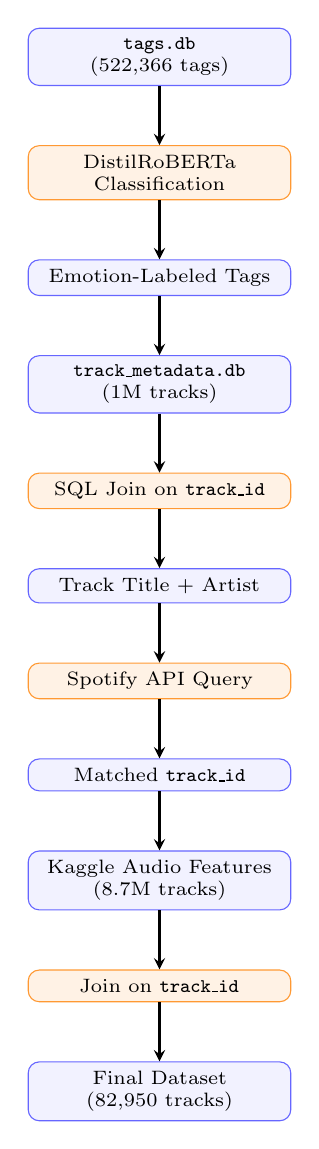
\begin{tikzpicture}[
    node distance=0.75cm,
    every node/.style={font=\scriptsize},
    data/.style={rectangle, draw=blue!60, fill=blue!5, rounded corners, text width=3.1cm, align=center, minimum height=0.8em},
    process/.style={rectangle, draw=orange!80, fill=orange!10, rounded corners, text width=3.1cm, align=center, minimum height=0.8em},
    arrow/.style={->, thick, >=stealth}
]

% Nodes
\node[data] (tagsdb) {\texttt{tags.db}\\(522,366 tags)};
\node[process, below=of tagsdb] (transformer) {DistilRoBERTa Classification};
\node[data, below=of transformer] (robertalabels) {Emotion-Labeled Tags};
\node[data, below=of robertalabels] (trackmeta) {\texttt{track\_metadata.db}\\(1M tracks)};
\node[process, below=of trackmeta] (joinmeta) {SQL Join on \texttt{track\_id}};
\node[data, below=of joinmeta] (trackinfo) {Track Title + Artist};
\node[process, below=of trackinfo] (spotifyquery) {Spotify API Query};
\node[data, below=of spotifyquery] (spotifyid) {Matched \texttt{track\_id}};
\node[data, below=of spotifyid] (kaggledb) {Kaggle Audio Features\\(8.7M tracks)};
\node[process, below=of kaggledb] (joinkaggle) {Join on \texttt{track\_id}};
\node[data, below=of joinkaggle] (finalset) {Final Dataset\\(82,950 tracks)};

% Arrows
\draw[arrow] (tagsdb) -- (transformer);
\draw[arrow] (transformer) -- (robertalabels);
\draw[arrow] (robertalabels) -- (trackmeta);
\draw[arrow] (trackmeta) -- (joinmeta);
\draw[arrow] (joinmeta) -- (trackinfo);
\draw[arrow] (trackinfo) -- (spotifyquery);
\draw[arrow] (spotifyquery) -- (spotifyid);
\draw[arrow] (spotifyid) -- (kaggledb);
\draw[arrow] (kaggledb) -- (joinkaggle);
\draw[arrow] (joinkaggle) -- (finalset);

\end{tikzpicture}
\caption{Emotion labeling and dataset construction pipeline.}
\label{fig:pipeline_final}
\end{figure}

\subsection{Data and Code Availability}
All data and code used in this study are available at: 

\url{https://github.com/macs30200-s23/course-project-VeraMao}.


\section{Results}
\subsection{Baseline Model Comparison}

To establish benchmark performance for multi-label music emotion classification, this study implemented and evaluated three commonly used classifiers: Multi-Layer Perceptron (MLP), Random Forest, and K-Nearest Neighbors (KNN). All models were trained on the same 12-dimensional audio feature set and evaluated using a top-$k$ dynamic matching strategy, where $k$ corresponds to the number of true labels per instance. This ensures a fairer assessment in the multi-label context and avoids penalizing models for predicting multiple relevant emotions.

\paragraph{Overall Performance.}
Among the three models, \textbf{Random Forest} achieved the highest micro-average F1 score (\textbf{0.6766}) and exact match accuracy (\textbf{36.67\%}). \textit{Exact match accuracy} refers to the proportion of instances for which the predicted emotion set exactly matches the true multilabel set. This is a strict metric in multi-label classification, and a score of 36.67\%, while seemingly modest, is considered relatively strong given the task's complexity and the presence of overlapping emotional labels.

\textbf{MLP} followed closely with an F1 score of 0.6757, benefiting from its ability to capture nonlinear interactions among features. In contrast, \textbf{KNN} underperformed across all metrics, particularly in exact match accuracy (30.30\%) and Hamming Loss (0.2565), likely due to its sensitivity to feature scaling and difficulty modeling sparse multilabel outputs in high-dimensional acoustic space.

\paragraph{Metric Rationale.}
Micro-averaged F1 score was selected as the primary evaluation metric because it accounts for all true positives, false positives, and false negatives across the dataset. Unlike macro F1, which treats all classes equally regardless of frequency, micro F1 provides a more balanced estimate in the presence of class imbalance, which is particularly relevant for music emotion classification where categories like \textit{joy} are overrepresented while \textit{fear} and \textit{disgust} are less common.

Hamming Loss was included to capture the average number of incorrect label assignments per sample. It penalizes both false positives and false negatives uniformly, offering a complementary view of model performance at the label level. A lower Hamming Loss indicates more precise multi-label predictions. In our results, Random Forest produced the lowest Hamming Loss (0.2261), reinforcing its advantage in minimizing unnecessary or missed predictions.

\begin{table}[H]
\centering
\caption{Overall performance metrics for three baseline classifiers under top-$k$ dynamic matching.}
\label{tab:model_comparison}
\begin{tabular}{lccccc}
\toprule
\textbf{Model} & \textbf{Micro F1} & \textbf{Exact Match (\%)} & \textbf{Hamming Loss} & \textbf{Macro F1} & \textbf{Weighted F1} \\
\midrule
Random Forest     & \textbf{0.6766} & \textbf{36.67} & \textbf{0.2261} & 0.5379 & 0.6547 \\
MLP               & 0.6757          & 36.27          & 0.2268          & 0.5187 & 0.6436 \\
KNN               & 0.6332          & 30.30          & 0.2565          & 0.5098 & 0.6188 \\
\bottomrule
\end{tabular}
\end{table}

\paragraph{Per-Class Analysis.}

As shown in Figure~\ref{fig:per_class_scores}, all models exhibit strong performance on high-frequency emotions like \textit{joy} and \textit{sadness}, with F1 scores exceeding 0.75 across classifiers. In contrast, minority or more ambiguous categories such as \textit{fear}, \textit{disgust}, and \textit{surprise} consistently receive much lower F1 scores—often below 0.40—regardless of model type.

This discrepancy is further clarified in Figure~\ref{fig:per_class_scores_rf}, which breaks down the Random Forest classifier’s precision, recall, and F1 by emotion. While precision remains moderately stable (typically 0.5–0.6) even for rare emotions, recall is significantly lower, indicating systematic under-prediction. For example, \textit{fear} achieves only 0.22 recall despite a precision of 0.55, and \textit{surprise} reaches just 0.28 recall.

Such imbalances between precision and recall highlight a key challenge in multilabel music emotion recognition: models tend to be conservative in assigning underrepresented labels, often missing relevant instances. These results align with prior findings on label imbalance and weak supervision in affective classification tasks \parencite{Ahsan2015, Tuba2025}.

For completeness, per-class performance matrices for KNN and MLP are provided in Appendix~\ref{appendix:per_class_heatmaps}. These additional visualizations reinforce the observed trend: minority classes suffer from limited recall and are often overshadowed by more frequently occurring emotions.

\begin{figure}[H]
\centering
\includegraphics[width=0.8\textwidth]{Graphics/F1 Score Per Emotion.png}
\caption{F1 score comparison across emotion categories for three models (Random Forest, MLP, KNN). Joy and Sadness are consistently well-predicted, while minority emotions like Fear and Disgust show much lower F1 performance.}
\label{fig:per_class_scores}
\end{figure}

\begin{figure}[H]
\centering
\includegraphics[width=0.8\textwidth]{Graphics/per_class_score/per_class_rf.png}
\caption{Per-class precision, recall, and F1-score for the Random Forest classifier. Joy and Sadness dominate predictive accuracy, while Fear and Surprise reveal low recall despite moderate precision.}
\label{fig:per_class_scores_rf}
\end{figure}


% \subsection{Random Forest Hyperparameter Optimization}

% While Random Forest already outperformed other baseline models in its default configuration, additional improvements were achieved through systematic hyperparameter tuning. I conducted a grid search across the following parameter ranges:

% \begin{itemize}
%     \item \texttt{n\_estimators}: \{100, 200\}
%     \item \texttt{max\_depth}: \{None, 10, 20\}
%     \item \texttt{min\_samples\_split}: \{2, 5\}
%     \item \texttt{min\_samples\_leaf}: \{1, 2\}
% \end{itemize}

% Using five-fold cross-validation and micro-average F1 as the evaluation metric, the best-performing parameter combination was:

% \begin{quote}
% \texttt{\{n\_estimators = 200, max\_depth = 20, min\_samples\_split = 2, min\_samples\_leaf = 1\}}
% \end{quote}

% \paragraph{Performance Gains.}
% The optimized Random Forest achieved a micro-average F1 score of \textbf{0.6794}, up from 0.6766 in the baseline. Exact match accuracy rose slightly to \textbf{36.95\%}, and Hamming Loss decreased to \textbf{0.2242}, indicating more precise multilabel predictions. Table~\ref{tab:rf_tuned_performance} summarizes key metrics.

% \begin{table}[H]
% \centering
% \begin{tabular}{|l|c|}
% \hline
% \textbf{Metric} & \textbf{Score} \\
% \hline
% Micro Precision & 0.6794 \\
% Micro Recall    & 0.6794 \\
% Micro F1 Score  & 0.6794 \\
% Exact Match Accuracy & 0.3695 \\
% Hamming Loss    & 0.2242 \\
% \hline
% \end{tabular}
% \caption{Evaluation metrics for optimized Random Forest model.}
% \label{tab:rf_tuned_performance}
% \end{table}

% \paragraph{Per-Class Improvements.}
% The optimized model maintained strong performance on high-frequency classes (\textit{joy}: F1 = 0.83; \textit{sadness}: F1 = 0.75) and modestly improved recognition of rare classes (e.g., \textit{fear}: F1 = 0.28; \textit{surprise}: F1 = 0.35). These F1 scores are computed against transformer-derived emotion labels, which were weakly assigned using a DistilRoBERTa classifier on Last.fm tags. While these labels are not ground truth in the traditional sense, they offer a consistent, semantically meaningful proxy for emotional content across a large-scale music corpus.

% Thus, the reported improvements should be interpreted as better alignment with the tag-based semantic emotion mapping pipeline, rather than human-annotated emotional ground truth. Nonetheless, the fact that tuning (e.g., deeper trees, more estimators) helps recover low-frequency emotions more accurately suggests the model is more robust to label sparsity and ambiguity.

% These results underscore the importance of careful hyperparameter tuning even for robust ensemble models, particularly when training on large, imbalanced, and noisily labeled datasets.

\subsection{Emotion Label Co-occurrence Patterns}

To elucidate structural dependencies within the multilabel annotation space, a pairwise co-occurrence matrix was computed across all emotion categories. As shown in Figure~\ref{fig:emotion_cooccur}, certain emotion pairs co-occur with high frequency, reflecting common affective blends in listener perceptions. Notably, \textit{joy} and \textit{sadness} co-occur in over 15,000 tracks, suggesting that many songs convey emotionally ambivalent or bittersweet tones. In contrast, combinations such as \textit{surprise} and \textit{fear} are comparatively rare, with fewer than 1,200 instances.

These patterns reveal several semantically proximal pairings—e.g., \textit{joy} and \textit{surprise}, or \textit{fear} and \textit{sadness}—that are prone to overlap, contributing to inter-label ambiguity. This ambiguity, in turn, may partially explain classifier confusion and low recall on minority categories. The findings underscore the importance of interpretability-driven evaluation in multi-emotion classification, especially for understanding errors arising from overlapping affective semantics.

\begin{figure}[H]
\centering
\includegraphics[width=\textwidth]{Graphics/Emotion_Co_Heatmap.pdf}
\caption{Co-occurrence matrix of emotion labels across multilabel annotations. Values reflect the number of tracks assigned each emotion pair.}
\label{fig:emotion_cooccur}
\end{figure}

\subsection{Global and Per-Label Feature Importance Analysis}

To assess how different architectures prioritize audio cues in multilabel classification, I computed global and class-specific feature importance across representative model types, including tree-based, distance-based, and neural network classifiers.

\paragraph{Methodology.} For linear and distance-based models, permutation importance was estimated using a \texttt{OneVsRestClassifier} wrapper and averaged over emotion classes. Tree-based models provided intrinsic importance values (\texttt{feature\_importances\_}), while neural architectures were interpreted via SHAP’s KernelExplainer applied to a stratified subsample of 100 training examples. Mean absolute SHAP values were used to quantify both global and emotion-specific contributions.

\begin{figure}[H]
\centering
\includegraphics[width=\textwidth]{Graphics/global_feature_importance_comparison.pdf}
\caption{Global feature importance scores across models. MLP importance computed via SHAP; Random Forest and KNN via permutation; Logistic Regression via normalized coefficients.}
\label{fig:feature_importance}
\end{figure}

As shown in Figure~\ref{fig:feature_importance}, Random Forest emphasized \texttt{acousticness}, \texttt{loudness}, and \texttt{energy}—features with sharp thresholds well-suited to tree-based decision boundaries. The high importance of \texttt{acousticness} (0.1214) aligns with its role in differentiating unplugged and high-arousal music, consistent with prior affective MIR findings \parencite{Huron2015, McCraty1998}.

KNN placed more weight on \texttt{danceability}, \texttt{valence}, and \texttt{mode}, suggesting that similarity-based classification is more influenced by rhythmic and tonal characteristics—features that likely produce tighter clusters in Euclidean space.

MLP showed more balanced attribution across features, reflecting its ability to capture nonlinear combinations. SHAP results indicated \texttt{speechiness}, \texttt{energy}, and \texttt{acousticness} as particularly influential. These dimensions may encode expressive subtleties (e.g., rap-like vocals or whispered tones) that are difficult for tree-based or distance-based models to capture.

Across all models, \texttt{key}, \texttt{mode}, and \texttt{time\_signature} consistently received low importance scores—consistent with the weak correlation patterns observed earlier. These features likely contribute little predictive value in large, genre-diverse datasets and may only matter in specialized musical contexts.

\paragraph{Per-Label Feature Importance.}
To examine model behavior at the class-specific level, I compared feature importance rankings for the emotion \textit{anger} across three classifiers—Random Forest, KNN, and MLP (SHAP-based).

\paragraph{Anger.}
All three models agree that \texttt{acousticness}, \texttt{loudness}, and \texttt{energy} are key predictors of \textit{anger}. Random Forest assigns the highest importance to \texttt{acousticness}, followed closely by \texttt{loudness} and \texttt{energy}, suggesting that anger is associated with low-acoustic, high-intensity audio signatures. KNN also emphasizes these features but disproportionately relies on \texttt{key} and \texttt{mode}, indicating sensitivity to tonal structure that may be confounded by genre or harmonic context. MLP, as revealed by SHAP values, distributes importance more diffusely, with \texttt{valence}, \texttt{acousticness}, and \texttt{loudness} emerging as modest contributors. The consistently high importance of \texttt{tempo} and \texttt{danceability} across models reinforces the link between anger and rhythmic drive.

\begin{figure}[H]
\centering
\includegraphics[width=\linewidth]{Graphics/per_label/anger_feature_importance.png}
\caption{Feature importance comparison for emotion: \textit{anger}.}
\label{fig:shap_anger}
\end{figure}

Feature importance profiles for the remaining emotions (\textit{disgust}, \textit{fear}, \textit{joy}, \textit{sadness}, and \textit{surprise}) are provided in Appendix~\ref{appendix:perlabel_importance}. These extended plots and comparisons reveal both shared and emotion-specific acoustic signatures. For instance, high-arousal features such as \texttt{energy} and \texttt{loudness} consistently appear among the top predictors for \textit{anger}, \textit{joy}, and \textit{surprise}, while low-valence emotions like \textit{fear} and \textit{sadness} are more strongly associated with \texttt{acousticness} and \texttt{valence}. Additionally, \texttt{speechiness} emerges as a reliable cue for \textit{disgust} and \textit{joy}, suggesting that lyrical or spoken-word content may play an outsized role in those categories. Conversely, features like \texttt{key}, \texttt{mode}, and \texttt{time\_signature} contribute minimally across all emotions, reinforcing earlier findings from the correlation and distributional analyses. Overall, these per-label comparisons help clarify which acoustic dimensions are broadly salient versus those that operate more selectively, thereby motivating the need for feature-wise ablation and error decomposition in later sections.

Together, these findings reinforce the value of per-label interpretation in multi-label settings. They demonstrate that while some features are broadly predictive, others contribute selectively, depending on the emotional context. This justifies the subsequent ablation and correlation-based redundancy analyses in the following.

\subsection{Feature Correlation Analysis}

To evaluate potential collinearity among the input variables, a Pearson correlation matrix was computed and visualized via heatmap (Figure~\ref{fig:feature_correlation}). This diagnostic offers insight into linear dependencies across audio features and informs subsequent steps in feature selection, normalization, and model interpretation.

Several strong correlations emerged. Most notably, \texttt{acousticness} exhibits substantial negative associations with both \texttt{energy} ($r = -0.72$) and \texttt{loudness} ($r = -0.58$), suggesting that acoustically rich tracks tend to be quieter and less energetic. Conversely, \texttt{energy} and \texttt{loudness} are strongly positively correlated ($r = 0.76$), consistent with psychophysical theories linking amplitude to perceived arousal. A moderate positive correlation between \texttt{danceability} and \texttt{valence} ($r = 0.55$) suggests that rhythmically engaging music is more likely to convey positive emotional valence.

In contrast, categorical or structural features such as \texttt{key}, \texttt{mode}, and \texttt{time\_signature} display weak or near-zero correlations with other variables. Their limited linear association implies that any emotional signal they encode likely arises through nonlinear interactions or genre-conditioned effects.

\begin{figure}[H]
\centering
\includegraphics[width=\textwidth]{Graphics/feature_correlation.png}
\caption{Pearson correlation matrix of the 12 Spotify audio features. High correlations indicate potential redundancy or shared perceptual dimensions.}
\label{fig:feature_correlation}
\end{figure}

These findings underscore the limitations of purely linear diagnostics in emotion modeling. To address potential non-additive and interaction-based effects, the modeling pipeline incorporates permutation-based and SHAP-based importance methods, which provide model-aware assessments of feature contributions.

\subsection{Ablation Study and Dimensionality Considerations}

To evaluate feature redundancy and quantify the marginal contribution of each acoustic variable, I conducted a stepwise ablation study using the Random Forest classifier. Features were removed iteratively in ascending order of global importance (as determined by the model’s global feature importance), and the classifier was retrained and evaluated at each step using the multilabel dynamic top-$k$ prediction framework.

\begin{table}[H]
\centering
\resizebox{\textwidth}{!}{
\begin{tabular}{|c|c|l|}
\hline
\textbf{Remaining Features} & \textbf{Accuracy} & \textbf{Dropped Features} \\
\hline
12 & 0.2403 & [] \\
11 & 0.2361 & [valence] \\
10 & 0.2361 & [valence, loudness] \\
9  & 0.2182 & [valence, loudness, instrumentalness] \\
8  & 0.2069 & [valence, loudness, instrumentalness, energy] \\
7  & 0.1904 & [valence, loudness, instrumentalness, energy, acousticness] \\
6  & 0.1890 & [valence, loudness, instrumentalness, energy, acousticness, danceability] \\
5  & 0.1932 & [valence, loudness, instrumentalness, energy, acousticness, danceability, speechiness] \\
4  & 0.1767 & [valence, loudness, instrumentalness, energy, acousticness, danceability, speechiness, liveness] \\
3  & 0.2201 & [\dots, tempo] \\
2  & 0.2347 & [\dots, key] \\
1  & 0.2370 & [\dots, mode] \\
\hline
\end{tabular}
}
\caption{Sequential ablation results. Features are removed based on ascending global importance. Accuracy reflects dynamic top-$k$ prediction performance.}
\label{tab:ablation_study}
\end{table}

\begin{figure}[H]
\centering
\includegraphics[width=0.75\textwidth]{Graphics/Ablation Study.png}
\caption{Impact of progressive feature removal on Random Forest classifier accuracy.}
\label{fig:ablation_study}
\end{figure}

Model accuracy decreased sharply upon removing the top five most informative features—\texttt{acousticness}, \texttt{energy}, \texttt{loudness}, \texttt{valence}, and \texttt{instrumentalness}—dropping from 0.2403 to 0.1767 with only four features retained. This trend highlights that emotional signal is concentrated in a core subset of high-importance acoustic dimensions.

Interestingly, slight performance recovery was observed after excluding low-importance features (e.g., \texttt{key}, \texttt{mode}, \texttt{time\_signature}), suggesting that these dimensions may introduce noise or irrelevant variance. These observations align with prior correlation and importance analyses that found minimal contribution from structural features.

\paragraph{PCA Considerations.} To further examine the role of dimensionality reduction, I retrained the Random Forest classifier using the original 12-feature input space without PCA transformation. This configuration yielded improved metrics: the micro-averaged F1 score increased to \textbf{0.690}, exact match accuracy rose to \textbf{38.77\%}, and Hamming Loss declined to \textbf{0.2166}. Gains were especially notable in underrepresented classes such as \textit{disgust} and \textit{fear}, where precision increased to 0.57.

These results indicate that PCA-based compression may inadvertently discard subtle, emotion-relevant variance that benefits fine-grained multilabel classification. Accordingly, all final models reported in this study employ the full, unreduced feature set.

\subsection{Per-Class Metrics and Misclassification Patterns}

Per-class performance varies substantially across emotion categories. To further examine systematic misclassifications, Figure~\ref{fig:confusion_rf} presents a heatmap for the Random Forest model. Notable error patterns include frequent confusion between \textit{Sadness} and \textit{Joy}, as well as underprediction of \textit{Fear} and \textit{Surprise}, both of which are often omitted entirely. These patterns suggest that certain emotional categories possess overlapping acoustic profiles or are more context-dependent, increasing classification difficulty.

\begin{figure}[H]
\centering
\includegraphics[width=\textwidth]{Graphics/misclassification_heatmap_random_forest.png}
\caption{Misclassification heatmap for the Random Forest model. Rows represent true emotion labels; columns represent predicted labels.}
\label{fig:confusion_rf}
\end{figure}

Additional misclassification heatmaps for KNN and MLP models are provided in Appendix~\ref{appendix:error_analysis_heatmaps}.

\subsection{Impact of Emotion Co-occurrence}

Emotion misclassification may also stem from multilabel co-occurrence effects. To investigate this, I computed the average number of co-labels per instance for each emotion and plotted it against that emotion’s false negative rate. As shown in Figure~\ref{fig:cooccur_missrate}, a clear inverse relationship emerges: emotions with higher co-occurrence, such as \textit{Surprise} and \textit{Fear}, tend to be missed more frequently. In contrast, \textit{Joy} is both distinctive and frequently isolated, yielding lower omission rates. This trend highlights a key challenge in multilabel classification: emotions embedded within complex affective contexts are more difficult to isolate during prediction.

\begin{figure}[H]
\centering
\includegraphics[width=0.6\textwidth]{Graphics/Error Analysis/Emotion Co vs Missed Prediction Rate.png}
\caption{Relationship between average emotion co-occurrence and false negative rate. Emotions that frequently appear alongside others (e.g., \textit{Surprise}, \textit{Fear}) are more likely to be entirely missed.}
\label{fig:cooccur_missrate}
\end{figure}

\subsection{SHAP-Based Interpretation of Misclassified Samples}

To investigate why certain emotions remain difficult to classify, I conducted a SHAP-based analysis on one misclassified instance per emotion. These samples were selected from predictions that fell just below their respective dynamic top-$k$ confidence thresholds. Each waterfall plot visualizes how audio features contributed to the model's decision, providing insight into failure mechanisms.

Figure~\ref{fig:shap_fear_waterfall} illustrates a misclassified \textit{fear} example with a predicted confidence of 0.124. SHAP values show that positive contributions from \texttt{speechiness} were neutralized by strong negative effects from \texttt{danceability}, \texttt{valence}, and \texttt{instrumentalness}. The low magnitude and contradictory directions of these contributions indicate the absence of a dominant predictive signal, resulting in indecision.

\begin{figure}[H]
\centering
\includegraphics[width=0.8\textwidth]{Graphics/shap_missed_labels/fear_missed_shap_waterfall.png}
\caption{SHAP explanation for misclassified \textit{Fear}. Contributions from key features failed to reach decision threshold.}
\label{fig:shap_fear_waterfall}
\end{figure}

In contrast, the misclassified \textit{joy} sample (Figure~\ref{fig:shap_joy_waterfall}) shows strong suppression by low \texttt{speechiness} and \texttt{tempo}, despite high values in \texttt{energy} and \texttt{danceability}. This highlights how absence of expected lyrical and rhythmic signals can override otherwise high-arousal acoustic profiles.

\begin{figure}[H]
\centering
\includegraphics[width=0.8\textwidth]{Graphics/shap_missed_labels/joy_missed_shap_waterfall.png}
\caption{SHAP explanation for misclassified \textit{Joy}. Negative contributions from low \texttt{speechiness} and \texttt{tempo} suppressed correct prediction.}
\label{fig:shap_joy_waterfall}
\end{figure}

SHAP analyses for the remaining emotions (\textit{anger}, \textit{disgust}, \textit{sadness}, \textit{surprise}) are provided in Appendix~\ref{appendix:shap_waterfalls}, with a typology of common failure modes summarized in Table~\ref{tab:failure_typology}.

\begin{table}[H]
\centering
\begin{tabular}{|l|l|p{8.5cm}|}
\hline
\textbf{Failure Mode} & \textbf{Emotion} & \textbf{Explanation} \\
\hline
Overlapping semantics & Sadness $\rightarrow$ Joy & Bittersweet or nostalgic tone interpreted as positive due to instrumentation \\
Lack of dominant cues & Fear & Weak signal across all features, leading to model indecision \\
Feature conflict & Disgust & Noisy combination of low valence but ambiguous rhythmic/timbral signals \\
Rhythmic mismatch & Anger, Joy & Tempo and time signature inconsistent with model prototype of class \\
Cultural encoding & Surprise & Subtle emotional valence varies by genre; high acousticness misinterpreted \\
\hline
\end{tabular}
\caption{Typology of common failure modes in multilabel music emotion classification.}
\label{tab:failure_typology}
\end{table}


\section{Discussion}

This study investigated how supervised machine learning models interpret Spotify-derived acoustic features when classifying songs into emotional categories, within a weakly supervised, multilabel framework. Beyond measuring performance, the analysis prioritized interpretability—focusing on both global feature importance and local explanation of prediction failures.

\textbf{Emotion-specific classification disparities.} Model performance was notably uneven across emotion categories. \textit{Joy} and \textit{Sadness} consistently achieved high F1 scores, while \textit{Fear}, \textit{Disgust}, and \textit{Surprise} remained error-prone. Heatmaps and label co-occurrence diagnostics suggest that such failures often stem from intrinsic ambiguity in the emotional signal, rather than model incapacity. For example, \textit{Fear} was frequently confused with both \textit{Sadness} and \textit{Joy}, likely due to overlapping acoustic profiles. This aligns with the observed inverse relationship between co-occurrence frequency and false negative rate: emotions that often appear in combination—such as \textit{Surprise} and \textit{Fear}—are more likely to be missed, suggesting that models struggle to isolate context-dependent affective cues.

\textbf{SHAP-based explanation of failure modes.} Local interpretability analyses revealed that many misclassifications arose not from strongly misleading features, but from diffuse, contradictory, or weak signals. In the case of \textit{Fear}, for instance, SHAP values across all features were near zero, leading to model indecision. These cases exemplify what might be called a “semantic vacuum,” in which the audio signal lacks a dominant pattern associated with a specific emotion. This finding, echoed in prior work on weakly supervised tags \parencite{Artemova2025, Kim2024}, reinforces the importance of considering emotional ambiguity as a first-class modeling challenge.

\textbf{Feature contribution and model heterogeneity.} Global importance scores identified perceptually salient features—such as \texttt{energy}, \texttt{valence}, and \texttt{acousticness}—as central to emotion inference. These align with established psychological models of arousal and positivity \parencite{Huron2015, McCraty1998}. However, models differed in how they utilized these cues: MLP distributed weights more evenly and captured nonlinear interactions, while KNN relied on cluster-inducing variables like \texttt{mode} and \texttt{danceability}, reflecting its sensitivity to local structure.

\textbf{Feature redundancy and robustness.} The ablation study showed that emotional prediction is driven by a compact but semantically rich feature subset. Removing the top five most informative features resulted in a 26\% drop in accuracy. Notably, performance partially rebounded when low-importance features—such as \texttt{key}, \texttt{mode}, and \texttt{time\_signature}—were removed, indicating that noise-prone or low-variance features may introduce instability. Correlation analysis confirmed that while \texttt{energy} and \texttt{loudness} are strongly correlated ($r = 0.76$), they contribute unique, nonlinear effects—supporting their joint inclusion despite collinearity.

\textbf{Failure typologies and cultural encoding.} SHAP analyses of misclassified samples revealed recurring patterns. For instance, \textit{Disgust} lacked consistent rhythmic or timbral anchors, while \textit{Surprise} was often misinterpreted as \textit{Sadness} or \textit{Fear} in genres with high \texttt{acousticness}, such as jazz. These cases suggest that cultural and genre-specific norms around emotional expression can confound audio-based inference, especially when models lack access to lyrical, historical, or listener context.

\textbf{Epistemological ambiguity in “error.”} Manual inspection of borderline cases complicates the notion of model failure. For instance, Billie Holiday’s \textit{All of Me} was labeled with \textit{Anger}, \textit{Sadness}, and \textit{Joy}, yet only \textit{Joy} was predicted. While technically incorrect, this prediction is arguably valid—underscoring a key limitation in multilabel music emotion modeling: the blurred boundary between algorithmic misclassification and human perceptual disagreement. Crowd-sourced or weakly labeled ground truth may reflect collective sentiment more than categorical truth.

\textbf{Methodological contributions.} Finally, the study illustrates the value of combining global and local interpretability tools. Permutation importance, SHAP waterfall plots, and co-occurrence diagnostics each revealed distinct failure mechanisms. This multi-angle approach offered insights that single-metric evaluation would have missed—particularly in diagnosing borderline, ambiguous, or context-dependent predictions. As such, interpretability emerges not just as a supplement to performance, but as a diagnostic lens critical for refining emotion-aware systems.

\subsection{Limitations}

Despite its contributions, this study has several limitations concerning label validity, feature representation, interpretability methods, and evaluation strategy.

The most fundamental limitation lies in the use of automatically generated emotion labels rather than human-annotated ground truth. Labels were inferred from a DistilRoBERTa classifier applied to Last.fm user tags, many of which are genre-descriptive, polysemous, or aesthetically focused (e.g., \textit{lo-fi}, \textit{dream pop}) rather than affective. While transformer-based tag-to-emotion mapping improves semantic coverage, its reliability for music emotion classification remains under-validated. This introduces the risk of semantic drift—where labels reflect inferred sentiment rather than listener-perceived emotion. Moreover, since the same weak labels were used for both model training and evaluation, performance metrics may reflect alignment with the labeling model rather than true generalization.

The use of a dynamic top-$k$ prediction threshold introduces further abstraction. Although it respects label cardinality and improves match quality, it imposes a hard cutoff that excludes borderline yet semantically plausible predictions. This especially penalizes ambiguous or co-occurring emotions such as \textit{fear} and \textit{surprise}, which often fall below the threshold despite moderate model confidence—compromising recall for minority classes.

The emotional taxonomy itself presents constraints. The six-class schema aligns with basic emotion theory but underrepresents the diversity and fluidity of musical affect. Music frequently conveys blended, evolving, or culturally-specific emotions that defy discrete categorization. Rigid label targets may therefore understate affective nuance. Future work should consider fuzzy labeling schemes or continuous representations (e.g., valence-arousal space) to better capture this complexity.

The fixed threshold of 0.8 for emotion label assignment also introduces bias. While this value prioritizes high-confidence tags and reduces semantic noise, it remains an arbitrary hyperparameter not systematically tuned. Appendix~\ref{appendix:threshold} reports a follow-up analysis suggesting that a 0.7 threshold offers improved label coverage—especially for underrepresented emotions like \textit{anger}, \textit{fear}, and \textit{surprise}. However, the downstream effects of threshold choice warrant further empirical validation via full relabeling and ablation studies.

Metadata limitations further constrain dataset completeness. Due to API mismatches, spelling inconsistencies, and missing Spotify metadata, many Last.fm tracks could not be matched. The final dataset of 82,950 songs overrepresents mainstream and Western music, limiting generalizability to niche genres or global musical traditions.

Feature representation also limits affective fidelity. Spotify’s 12 audio features capture coarse acoustic properties but omit structural, lyrical, and cultural cues—such as melodic contour, harmonic tension, and lyrical sentiment—that shape listener emotion. As a result, models may over-rely on surface-level features (e.g., \texttt{loudness}, \texttt{tempo}) whose emotional interpretation is genre-dependent. For instance, high \texttt{acousticness} may connote intimacy in folk but surprise or playfulness in jazz.

The interpretability tools used in this study, though valuable, have technical constraints. SHAP’s KernelExplainer is computationally intensive and requires small reference sets, limiting scalability. SHAP values are also sensitive to feature collinearity—making importance scores less stable when features like \texttt{energy} and \texttt{loudness} co-vary. Moreover, axis-aligned models like Random Forests may overemphasize certain features due to their split mechanics, complicating cross-model comparisons.

Dimensionality reduction (e.g., PCA) was intentionally excluded to preserve interpretability. While this helped retain signals for rare emotions such as \textit{disgust}, it may have also preserved noisy or redundant features. Future pipelines could benefit from SHAP-guided pruning or domain-aware selection to balance interpretability and robustness.

The evaluation strategy itself is impacted by labeling incompleteness. Since many songs carry only partial emotion tags, true positive predictions may be penalized as false positives. This weakens the interpretability of metrics like F1 and Exact Match, especially for songs with multilayered or genre-dependent emotional content.

Finally, cultural and stylistic biases embedded in both the training tags and model predictions remain unresolved. Tags such as “dark ambient” may be mapped to \textit{fear} or \textit{sadness}, although the user’s intent may be aesthetic, not emotional. Likewise, genre conventions shape how emotions are acoustically encoded—yet current features are not designed to capture cross-cultural affective variation. Without genre-aware modeling or cultural grounding, classifiers risk overfitting to dominant musical norms and failing to generalize meaningfully.

Addressing these limitations will require multimodal inputs (e.g., lyrics, harmonic embeddings, listener surveys), genre- and culture-aware model designs, and benchmark datasets with verified annotations. Integrating human coding into the labeling pipeline and evaluating sensitivity to threshold and taxonomic design will be essential for building more valid and inclusive emotion recognition systems.

\section{Conclusion}

This study examined the extent to which supervised machine learning models can classify musical emotion using only Spotify-derived acoustic features. Leveraging a weakly supervised labeling pipeline—where emotion labels were inferred from Last.fm tags via a DistilRoBERTa transformer—the resulting dataset enabled multilabel classification across six basic emotions: anger, disgust, fear, joy, sadness, and surprise.

Among the models evaluated (Random Forest, Logistic Regression, K-Nearest Neighbors, and Multi-Layer Perceptron), Random Forest achieved the highest micro-average F1 and exact match scores. This performance likely reflects both its suitability for thresholdable, high-variance features (e.g., \texttt{acousticness}, \texttt{energy}, \texttt{loudness}) and its advantage from full hyperparameter tuning. However, model performance varied substantially by emotion: \textit{Joy} and \textit{Sadness} were consistently predicted with high confidence, whereas \textit{Fear}, \textit{Disgust}, and \textit{Surprise} posed persistent challenges—often due to low acoustic salience, semantic overlap, and frequent co-occurrence with other emotions.

Interpretability emerged as a key analytical lens. Global feature importance scores revealed divergent inductive biases: Random Forest favored separable, high-variance features; MLPs leveraged nonlinear feature combinations; KNN relied on local clustering. SHAP-based local interpretations revealed that many misclassifications stemmed not from erroneous inputs but from ambiguous or weakly expressive acoustic profiles—highlighting the challenge of modeling fuzzy affective categories from audio alone.

The ablation study confirmed the predictive centrality of a small set of perceptually salient features. Removal of top contributors—\texttt{acousticness}, \texttt{energy}, \texttt{valence}, among others—led to a substantial accuracy drop, underscoring their role in affective inference. At the same time, the elimination of weak or noisy features (e.g., \texttt{key}, \texttt{mode}) modestly improved robustness, suggesting that excessive feature inclusion may hinder generalization.

Several limitations warrant caution. The emotion labels were inferred rather than empirically annotated, introducing potential biases from genre conventions or tag semantics. Top-$k$ prediction thresholds improved interpretability but suppressed emotional plurality, especially for minority or co-labeled emotions like \textit{Fear} and \textit{Surprise}. Metadata mismatches and API failures further constrained dataset completeness, potentially skewing the corpus toward English-language and Western musical traditions. Finally, SHAP explanations—while insightful—remain sensitive to model architecture and training dynamics, limiting direct cross-model comparisons.

Despite these constraints, the study affirms that Spotify audio features encode meaningful emotional structure. Yet, acoustic data alone is insufficient for high-fidelity emotion classification. Future research should adopt a multimodal framework, integrating lyrics, melodic contour, harmonic progression, and temporal structure. Emotion annotations should reflect probabilistic, fuzzy, or listener-rated constructs rather than discrete labelings. Cross-cultural and genre-aware model design will also be crucial to ensure generalizability and inclusivity.

In sum, while supervised learning over acoustic features offers a promising foundation for music emotion recognition, achieving deeper affective fidelity demands models that move beyond sound—toward context, semantics, and human subjectivity. Doing so not only improves classification fidelity, but also enhances the utility of emotion-aware systems in downstream applications such as personalized music recommendation, affective computing, music therapy, and cultural analytics.


\newpage
\printbibliography
\newpage

\appendix

\section{Transformer Score Threshold Justification}
\label{appendix:threshold}

To determine an appropriate threshold for emotion label assignment from transformer-based tag scores, I conducted a descriptive analysis using the output of the DistilRoBERTa classifier applied to Last.fm tags. As shown in Figure~\ref{fig:maxscore_hist}, the distribution of maximum emotion scores per tag is highly right-skewed, with the majority of tags receiving relatively low confidence scores. This indicates that a high threshold (e.g., $0.8$ or above) may excessively filter out potentially meaningful emotional information.

\begin{figure}[H]
\centering
\includegraphics[width=0.8\textwidth]{Graphics/Appendix/Distribution of Max Emotion Scores Per Tag.png}
\caption{Distribution of maximum emotion scores per tag above threshold 0.5.}
\label{fig:maxscore_hist}
\end{figure}

\FloatBarrier

I further evaluated the number of tags retained under various thresholds ranging from $0.5$ to $0.9$ (Figure~\ref{fig:threshold_line}). At a threshold of $0.8$, only around 41,000 tags remain, while at $0.7$, over 58,000 tags are preserved—representing a substantial increase in usable emotional annotations without introducing a large volume of low-confidence data.

\begin{figure}[H]
\centering
\includegraphics[width=0.8\textwidth]{Graphics/Appendix/Number of Tags Retianed by Threshold.png}
\caption{Line Plot Number of Tags Retained by Threshold}
\label{fig:threshold_line}
\end{figure}
\FloatBarrier

Importantly, while joy and sadness dominate across all thresholds, lowering the threshold from $0.8$ to $0.7$ leads to substantially improved representation of minority emotions such as anger, surprise, and fear. As shown in Appendix Figures~\ref{fig:threshold_0.6}, \ref{fig:threshold_0.7}, and~\ref{fig:threshold_0.8}, the number of tags assigned to these minority categories increases significantly at lower thresholds without completely distorting the underlying class distribution. Specifically, threshold $0.7$ provides a more balanced compromise, retaining the major emotion categories while enabling inclusion of less frequently predicted emotions.

By contrast, a threshold of $0.6$ (Appendix Figure~\ref{fig:threshold_0.6}) introduces a noticeable shift in distribution that may reflect higher label noise, potentially due to the inclusion of tags with lower classifier confidence. This is consistent with the long-tail pattern observed in the score histogram (Figure~\ref{fig:maxscore_hist}). 

\begin{figure}[h]
  \centering
  \includegraphics[width=0.6\textwidth]{Graphics/Appendix/0.6 Threshold.png}
  \caption{Emotion label distribution at threshold $=0.6$.}
  \label{fig:threshold_0.6}
\end{figure}

\begin{figure}[h]
  \centering
  \includegraphics[width=0.6\textwidth]{Graphics/Appendix/0.7 Threshold.png}
  \caption{Emotion label distribution at threshold $=0.7$.}
  \label{fig:threshold_0.7}
\end{figure}

\begin{figure}[h]
  \centering
  \includegraphics[width=0.6\textwidth]{Graphics/Appendix/0.8 Threshold.png}
  \caption{Emotion label distribution at threshold $=0.8$.}
  \label{fig:threshold_0.8}
\end{figure}

To evaluate the impact of emotion classification threshold on downstream model performance, we compared the predictive results of three multi-label classifiers (MLP, Random Forest, and KNN) trained on datasets labeled with thresholds of $0.7$ and $0.8$. As shown in Table~\ref{tab:threshold_comparison}, both thresholds yielded similar micro-average F1 scores across models, indicating consistent overall accuracy. However, threshold $0.7$ demonstrated several advantages.

First, the 0.7-labeled dataset achieved slightly higher micro F1 scores on MLP and KNN (0.6725 and 0.6350) compared to their 0.8-labeled counterparts (0.6757 and 0.6332), and comparable performance on Random Forest (0.6757 vs. 0.6766). Second, the exact match accuracy—a strict metric measuring full-label agreement—was marginally higher for all three models under threshold 0.7. Notably, the Random Forest model achieved an exact match accuracy of $0.3690$ with $0.7$ threshold, compared to $0.3667$ under $0.8$.

More importantly, per-class F1 scores showed improved recall for minority emotions such as \textit{disgust}, \textit{fear}, and \textit{surprise} under the $0.7$ setting, suggesting that this threshold supports better emotion diversity in label distribution. For example, MLP's F1-score for \textit{fear} increased from $0.25$ to $0.28$, and \textit{disgust} from $0.40$ to $0.38$ despite the trade-off in precision.

\begin{table}[H]
\centering
\caption{Comparison of Micro F1 and Exact Match Accuracy under Different Labeling Thresholds}
\label{tab:threshold_comparison}
\begin{tabular}{lcccc}
\toprule
\textbf{Model} & \textbf{Threshold} & \textbf{Micro F1} & \textbf{Exact Match} & \textbf{Hamming Loss} \\
\midrule
MLP & 0.7 & 0.6725 & 0.3580 & 0.2282 \\
MLP & 0.8 & 0.6757 & 0.3627 & 0.2268 \\
RF  & 0.7 & 0.6757 & 0.3690 & 0.2259 \\
RF  & 0.8 & 0.6766 & 0.3667 & 0.2261 \\
KNN & 0.7 & 0.6350 & 0.3075 & 0.2543 \\
KNN & 0.8 & 0.6332 & 0.3030 & 0.2565 \\
\bottomrule
\end{tabular}
\end{table}

In summary, while threshold $0.8$ yields marginally cleaner labels with high confidence, threshold $0.7$ offers a better trade-off between label richness, minority emotion coverage, and predictive performance. Therefore, for future iterations of this classification pipeline, I recommend adopting a threshold of $0.7$.

\newpage

\section{Raw Dataset Summary Statistics}
\label{app:rawdata}

\begin{table}[H]
\centering
\resizebox{\textwidth}{!}{
\begin{tabular}{|l|r|r|r|r|r|r|r|r|}
\hline
\textbf{Feature} & \textbf{Count} & \textbf{Mean} & \textbf{Std} & \textbf{Min} & \textbf{25\%} & \textbf{50\%} & \textbf{75\%} & \textbf{Max} \\
\hline
Acousticness & 82,950 & 0.240 & 0.304 & 0.000 & 0.004 & 0.079 & 0.409 & 0.996 \\
Danceability & 82,950 & 0.521 & 0.175 & 0.000 & 0.397 & 0.525 & 0.648 & 0.980 \\
Energy & 82,950 & 0.653 & 0.249 & 0.000 & 0.476 & 0.696 & 0.868 & 1.000 \\
Instrumentalness & 82,950 & 0.155 & 0.290 & 0.000 & 0.000 & 0.001 & 0.114 & 0.993 \\
Key & 82,950 & 5.328 & 3.562 & 0.000 & 2.000 & 5.000 & 9.000 & 11.000 \\
Liveness & 82,950 & 0.196 & 0.160 & 0.009 & 0.095 & 0.130 & 0.258 & 1.000 \\
Loudness (dB) & 82,950 & -8.664 & 4.338 & -50.014 & -10.943 & -7.779 & -5.537 & 3.744 \\
Mode & 82,950 & 0.653 & 0.476 & 0.000 & 0.000 & 1.000 & 1.000 & 1.000 \\
Speechiness & 82,950 & 0.074 & 0.079 & 0.000 & 0.034 & 0.045 & 0.076 & 0.960 \\
Tempo (BPM) & 82,950 & 122.38 & 29.48 & 0.000 & 99.85 & 120.11 & 140.19 & 219.93 \\
Time Signature & 82,950 & 3.905 & 0.393 & 0.000 & 4.000 & 4.000 & 4.000 & 5.000 \\
Valence & 82,950 & 0.479 & 0.258 & 0.000 & 0.265 & 0.470 & 0.689 & 0.989 \\
\hline
\end{tabular}
}
\caption{Descriptive statistics for 12 Spotify audio features across 82,950 records in the raw dataset.}
\label{tab:eda-summary}
\end{table}

\newpage

\section{Boxplots of Acoustic Features by Emotion Category}
\label{appendix:feature_distributions}

\begin{figure}[H]
\centering
\includegraphics[width=0.9\textwidth]{Graphics/feature_by_emotion/danceability_by_emotion_boxplot.png}
\caption{Distribution of \texttt{danceability} by emotion category.}
\end{figure}

\begin{figure}[H]
\centering
\includegraphics[width=0.9\textwidth]{Graphics/feature_by_emotion/instrumentalness_by_emotion_boxplot.png}
\caption{Distribution of \texttt{instrumentalness} by emotion category.}
\end{figure}

\begin{figure}[H]
\centering
\includegraphics[width=0.9\textwidth]{Graphics/feature_by_emotion/key_by_emotion_boxplot.png}
\includegraphics[width=0.9\textwidth]{Graphics/feature_by_emotion/mode_by_emotion_boxplot.png}
\caption{Distribution of \texttt{key} and \texttt{mode} by emotion category.}
\end{figure}

\begin{figure}[H]
\centering
\includegraphics[width=0.9\textwidth]{Graphics/feature_by_emotion/liveness_by_emotion_boxplot.png}
\caption{Distribution of \texttt{liveness} by emotion category.}
\end{figure}

\begin{figure}[H]
\centering
\includegraphics[width=0.9\textwidth]{Graphics/feature_by_emotion/loudness_by_emotion_boxplot.png}
\caption{Distribution of \texttt{loudness} by emotion category.}
\end{figure}

\begin{figure}[H]
\centering
\includegraphics[width=0.9\textwidth]{Graphics/feature_by_emotion/speechiness_by_emotion_boxplot.png}
\caption{Distribution of \texttt{speechiness} by emotion category.}
\end{figure}

\begin{figure}[H]
\centering
\includegraphics[width=0.9\textwidth]{Graphics/feature_by_emotion/tempo_by_emotion_boxplot.png}
\includegraphics[width=0.9\textwidth]{Graphics/feature_by_emotion/time_signature_by_emotion_boxplot.png}
\caption{Distribution of \texttt{tempo} and \texttt{time signature} by emotion category.}
\end{figure}

\newpage

\section{Per-Class Performance Metrics (KNN and MLP)}
\label{appendix:per_class_heatmaps}

% === KNN
\paragraph{K-Nearest Neighbors (KNN).}
As shown in Figure~\ref{fig:per_class_knn}, KNN achieved high recall and F1-score for \textit{Joy} and \textit{Sadness}, but struggled significantly on low-frequency emotions such as \textit{Fear} and \textit{Disgust}.

\begin{figure}[H]
\centering
\includegraphics[width=0.8\textwidth]{Graphics/per_class_score/per_class_knn.png}
\caption{Per-class metrics for K-Nearest Neighbors classifier.}
\label{fig:per_class_knn}
\end{figure}

% === MLP
\paragraph{Multi-Layer Perceptron (MLP).}
Figure~\ref{fig:per_class_mlp} shows that the MLP slightly improved over KNN for minority emotions, though recall remained low for \textit{Fear} and \textit{Surprise}.

\begin{figure}[H]
\centering
\includegraphics[width=0.8\textwidth]{Graphics/per_class_score/per_class_mlp.png}
\caption{Per-class metrics for Multi-Layer Perceptron classifier.}
\label{fig:per_class_mlp}
\end{figure}

\FloatBarrier

\newpage

\section{Per-Label Feature Importance by Emotion Category}
\label{appendix:perlabel_importance}

To complement the global feature analysis, I examined per-label feature importance across all six emotion categories using Random Forest, KNN, and SHAP-based MLP classifiers. Visualizations and discussions for each emotion are presented below.

\paragraph{Disgust.} For \textit{disgust}, all models highlight \texttt{speechiness}, \texttt{acousticness}, and \texttt{valence} as important predictors. Random Forest places the greatest weight on \texttt{speechiness} (0.117), suggesting that vocal texture—such as harsh or spoken delivery—may convey disgust. KNN agrees on this ranking but assigns relatively high importance to \texttt{mode} and \texttt{key}, indicating a possible reliance on harmonic context that may reflect genre patterns more than affective signals. MLP SHAP values, although smaller in magnitude, still elevate \texttt{speechiness} and \texttt{danceability}, reinforcing the notion that disgust is acoustically expressed through rhythmic and vocal cues rather than tonal structure. Compared to emotions like \textit{joy} or \textit{sadness}, feature contributions for \textit{disgust} appear more evenly distributed, which may reflect the emotion’s more context-dependent or ambiguous nature in music.

\begin{figure}[H]
\centering
\includegraphics[width=\linewidth]{Graphics/per_label/disgust_feature_importance.png}
\caption{Feature importance (MLP SHAP) for emotion: \textit{disgust}}
\label{fig:shap_disgust}
\end{figure}

\paragraph{Fear.} For \textit{fear}, models show consistent reliance on \texttt{valence}, \texttt{loudness}, and \texttt{energy}, aligning with psychological literature that defines fear as a low-valence, high-arousal emotion. Random Forest assigns highest importance to \texttt{valence} (0.111) and \texttt{loudness} (0.108), suggesting that low-intensity, dark, or ambiguous tracks are indicative of fear responses. KNN emphasizes similar features but also places considerable weight on \texttt{mode} and \texttt{instrumentalness}, potentially capturing modal dissonance or texture typical in suspenseful music. In contrast, MLP assigns relatively flat SHAP scores across features, with slightly higher values for \texttt{valence}, \texttt{energy}, and \texttt{liveness}. This indicates that MLP struggles to isolate dominant acoustic signals for \textit{fear}, which may help explain its poor classification performance on this category. The absence of strong, consistent cues likely reflects the contextual and genre-dependent nature of fear in music.

\begin{figure}[H]
\centering
\includegraphics[width=\linewidth]{Graphics/per_label/fear_feature_importance.png}
\caption{Feature importance (MLP SHAP) for emotion: \textit{fear}}
\label{fig:shap_fear}
\end{figure}

\paragraph{Joy.} Across all models, \texttt{speechiness} emerges as the most important feature for predicting \textit{joy}. This suggests that joyful songs often involve pronounced lyrical or spoken-word elements—consistent with upbeat, expressive vocal delivery. Random Forest assigns the highest weight to \texttt{speechiness} , followed by \texttt{acousticness}, \texttt{tempo}, and \texttt{danceability}, indicating that timbral brightness and rhythmic energy are jointly predictive of positive affect. KNN highlights similar features but with reduced magnitude, and additionally emphasizes \texttt{mode} and \texttt{key}, aligning with traditional tonal-emotion mappings that associate major keys with happiness. In contrast, MLP SHAP values show \texttt{speechiness} as most predictive, with moderate contributions from \texttt{energy} and \texttt{valence}. These differences reflect MLP's tendency to spread importance across features and learn subtle nonlinear combinations. The convergence across models underscores the reliability of rhythmic and vocal cues in signaling musical joy.

\begin{figure}[H]
\centering
\includegraphics[width=\linewidth]{Graphics/per_label/joy_feature_importance.png}
\caption{Feature importance (MLP SHAP) for emotion: \textit{joy}}
\label{fig:shap_joy}
\end{figure}

\paragraph{Sadness.} All three models consistently rank \texttt{energy} as the most influential feature for classifying \textit{sadness}, supporting the view that lower energy levels are a hallmark of melancholic or reflective tracks. Random Forest assigns high importance to \texttt{speechiness}, \texttt{acousticness}, and \texttt{loudness}, indicating that soft, lyric-rich, and minimally amplified compositions are common among sad songs. SHAP values from the MLP model highlight a similar trend, especially the heightened role of \texttt{energy} (0.078), reinforcing that reduced dynamic intensity is predictive of sadness. KNN also places moderate emphasis on \texttt{tempo}, \texttt{valence}, and \texttt{danceability}, although its importance scores are more diffuse. Interestingly, all models treat \texttt{mode} and \texttt{time\_signature} as minimally informative, suggesting that formal tonal structure plays a limited role in sadness detection within this dataset. These patterns collectively affirm the acoustic softness and emotional introspection typically associated with sad musical affect.

\begin{figure}[H]
\centering
\includegraphics[width=\linewidth]{Graphics/per_label/sadness_feature_importance.png}
\caption{Feature importance (MLP SHAP) for emotion: \textit{sadness}}
\label{fig:shap_sadness}
\end{figure}

\paragraph{Surprise.} For \textit{surprise}, all three models converge on a core set of predictive features—namely, \texttt{loudness}, \texttt{tempo}, \texttt{danceability}, and \texttt{energy}. Random Forest assigns nearly equal importance to this cluster of high-arousal descriptors, suggesting that \textit{surprise} is encoded through dynamic intensity and rhythmic drive. KNN reinforces this trend with elevated weights on \texttt{tempo} and \texttt{valence}, while also placing substantial emphasis on \texttt{mode} and \texttt{key}—potentially overfitting to harmonic novelty. The MLP model, via SHAP analysis, identifies moderate importance for \texttt{loudness} and \texttt{energy} but shows flatter distributions overall, implying more diffuse activation in non-linear interactions. Notably, all models deem \texttt{speechiness} and \texttt{instrumentalness} less critical, perhaps reflecting that lyrics and texture are secondary to rhythmic and intensity cues when detecting musical surprise. These patterns align with prior work linking \textit{surprise} to heightened arousal and irregular structural transitions in music.

\begin{figure}[H]
\centering
\includegraphics[width=\linewidth]{Graphics/per_label/surprise_feature_importance.png}
\caption{Feature importance (MLP SHAP) for emotion: \textit{surprise}}
\label{fig:shap_surprise}
\end{figure}

\newpage

\section{Supplementary Misclassification Heatmaps}
\label{appendix:error_analysis_heatmaps}

Figures~\ref{fig:confusion_knn} and~\ref{fig:confusion_mlp} visualize misclassification patterns for the KNN and MLP models. Error distributions resemble those seen in the Random Forest classifier, with consistent confusion between semantically close emotions.

\begin{figure}[H]
\centering
\includegraphics[width=\textwidth]{Graphics/misclassification_heatmap_knn.png}
\caption{Misclassification heatmap for the KNN model. \textit{Sadness} is frequently confused with \textit{Joy} and \textit{Fear}.}
\label{fig:confusion_knn}
\end{figure}

\begin{figure}[H]
\centering
\includegraphics[width=\textwidth]{Graphics/misclassification_heatmap_mlp.png}
\caption{Misclassification heatmap for the MLP model. Similar to KNN, common misclassifications occur between \textit{Sadness}, \textit{Joy}, and \textit{Fear}.}
\label{fig:confusion_mlp}
\end{figure}

\newpage

\section{SHAP Waterfall Visualizations for Misclassified Emotions}
\label{appendix:shap_waterfalls}

\textbf{Anger}: The model predicted a confidence score of 0.583 but still fell short of the top-$k$ cutoff. High \texttt{energy} and low \texttt{valence} were positively associated with anger—consistent with aggressive delivery and negative emotional tone. However, low \texttt{tempo} and abnormal \texttt{time\_signature} contributed negatively, suggesting rhythmic ambiguity may mask anger cues.

\begin{figure}[H]
\centering
\includegraphics[width=0.8\textwidth]{Graphics/shap_missed_labels/anger_missed_shap_waterfall.png}
\caption{SHAP explanation for misclassified \textit{Anger}.}
\label{fig:shap_anger_waterfall}
\end{figure}

\textbf{Disgust}: Moderate \texttt{speechiness}, \texttt{energy}, and low \texttt{valence} were aligned with disgust, but weak contributions from \texttt{loudness} and \texttt{danceability}, and negative influence from \texttt{instrumentalness}, indicate that disgust lacks consistent acoustic signatures.

\begin{figure}[H]
\centering
\includegraphics[width=0.8\textwidth]{Graphics/shap_missed_labels/disgust_missed_shap_waterfall.png}
\caption{SHAP explanation for misclassified \textit{Disgust}.}
\label{fig:shap_disgust_waterfall}
\end{figure}

\textbf{Sadness}: Surprisingly, low \texttt{tempo} and \texttt{energy} pushed the score downward. Although expected to correlate with sadness, the model may rely more heavily on \texttt{acousticness} or \texttt{instrumentalness}, which were absent in this case.
\FloatBarrier

\begin{figure}[H]
\centering
\includegraphics[width=0.8\textwidth]{Graphics/shap_missed_labels/sadness_missed_shap_waterfall.png}
\caption{SHAP explanation for misclassified \textit{Sadness}.}
\label{fig:shap_sadness_waterfall}
\end{figure}

\textbf{Surprise}: Despite moderate \texttt{loudness}, \texttt{mode}, and \texttt{danceability}, high \texttt{acousticness} suppressed the prediction. This suggests the model interpreted the track as introspective rather than surprising, highlighting ambiguity in acoustic cues.

\begin{figure}[H]
\centering
\includegraphics[width=0.8\textwidth]{Graphics/shap_missed_labels/surprise_missed_shap_waterfall.png}
\caption{SHAP explanation for misclassified \textit{Surprise}.}
\label{fig:shap_surprise_waterfall}
\end{figure}
\FloatBarrier


\end{document}
